%%%%%%%%%%%%%%%%%%%%%%%%%%%%%%%%%%%%%%%%%
% Beamer Presentation
% LaTeX Template
% Version 1.0 (10/11/12)
%
% This template has been downloaded from:
% http://www.LaTeXTemplates.com
%
% License:
% CC BY-NC-SA 3.0 (http://creativecommons.org/licenses/by-nc-sa/3.0/)
%
%%%%%%%%%%%%%%%%%%%%%%%%%%%%%%%%%%%%%%%%%

%----------------------------------------------------------------------------------------
%	PACKAGES AND THEMES
%----------------------------------------------------------------------------------------

\documentclass{beamer}

\mode<presentation> {

% The Beamer class comes with a number of default slide themes
% which change the colors and layouts of slides. Below this is a list
% of all the themes, uncomment each in turn to see what they look like.

%\usetheme{default}
%\usetheme{AnnArbor}
%\usetheme{Antibes}
%\usetheme{Bergen}
%\usetheme{Berkeley}
%\usetheme{Berlin}
%\usetheme{Boadilla}
%\usetheme{CambridgeUS}
%\usetheme{Copenhagen}
%\usetheme{Darmstadt}
%\usetheme{Dresden}
%\usetheme{Frankfurt}
%\usetheme{Goettingen}
%\usetheme{Hannover}
%\usetheme{Ilmenau}
%\usetheme{JuanLesPins}
%\usetheme{Luebeck}
%\usetheme{Madrid}
\usetheme{Malmoe}
%\usetheme{Marburg}
%\usetheme{Montpellier}
%\usetheme{PaloAlto}
%\usetheme{Pittsburgh}
%\usetheme{Rochester}
%\usetheme{Singapore}
%\usetheme{Szeged}
%\usetheme{Warsaw}

% As well as themes, the Beamer class has a number of color themes
% for any slide theme. Uncomment each of these in turn to see how it
% changes the colors of your current slide theme.

%\usecolortheme{albatross}
%\usecolortheme{beaver}
%\usecolortheme{beetle}
%\usecolortheme{crane}
%\usecolortheme{dolphin}
%\usecolortheme{dove}
%\usecolortheme{fly}
%\usecolortheme{lily}
%\usecolortheme{orchid}
%\usecolortheme{rose}
%\usecolortheme{seagull}
%\usecolortheme{seahorse}
%\usecolortheme{whale}
%\usecolortheme{wolverine}

%\setbeamertemplate{footline} % To remove the footer line in all slides uncomment this line
%\setbeamertemplate{footline}[page number] % To replace the footer line in all slides with a simple slide count uncomment this line

%\setbeamertemplate{navigation symbols}{} % To remove the navigation symbols from the bottom of all slides uncomment this line
}

\usepackage{graphicx} % Allows including images
\usepackage{booktabs} % Allows the use of \toprule, \midrule and \bottomrule in tables
\usepackage{pdfpages}

%----------------------------------------------------------------------------------------
%	TITLE PAGE
%----------------------------------------------------------------------------------------

\title[Group 5 - MySL]{MySL} % The short title appears at the bottom of every slide, the full title is only on the title page

\author{Rafael Aldana - Vincent Delitz - Ruth Eriksson} % Your name
\institute[] % Your institution as it will appear on the bottom of every slide, may be shorthand to save space
{
ID2216 Developing Mobile Applications\\ % Your institution for the title page
\medskip
\textit{Group 5 - Project presentation} % Your email address
}
\date{\today} % Date, can be changed to a custom date

\begin{document}

\begin{frame}
\titlepage % Print the title page as the first slide
\end{frame}

\begin{frame}
\frametitle{Overview} % Table of contents slide, comment this block out to remove it
\tableofcontents % Throughout your presentation, if you choose to use \section{} and \subsection{} commands, these will automatically be printed on this slide as an overview of your presentation
\end{frame}

%----------------------------------------------------------------------------------------
%	PRESENTATION SLIDES
%----------------------------------------------------------------------------------------

%------------------------------------------------

\section{Domain of interest} % Sections can be created in order to organize your presentation into discrete blocks, all sections and subsections are automatically printed in the table of contents as an overview of the talk

\begin{frame}
\frametitle{Domain of interest} % Table of contents slide, comment this block out to remove it
\begin{itemize}
\item SL travellers might not make the most of the SL card
\item 3/7-day passes are more expensive than 30/90-day passes
\item Posts on the internet are not standardized
\end{itemize}
\end{frame}

%------------------------------------------------

\begin{frame}
\frametitle{Domain of interest} % Table of contents slide, comment this block out to remove it
The proposed app:
\begin{itemize}
\item standardizes post/request parameters regarding the SL card
\item enables post/request matching to make contact easier
\end{itemize}
\end{frame}

%------------------------------------------------

\section{WebApp prototype} % Sections can be created in order to organize your presentation into discrete blocks, all sections and subsections are automatically printed in the table of contents as an overview of the talk

%------------------------------------------------

\subsection{Paper prototype} % A subsection can be created just before a set of slides with a common theme to further break down your presentation into chunks

%------------------------------------------------

\begin{frame}
\frametitle{Paper prototype}
\begin{figure}
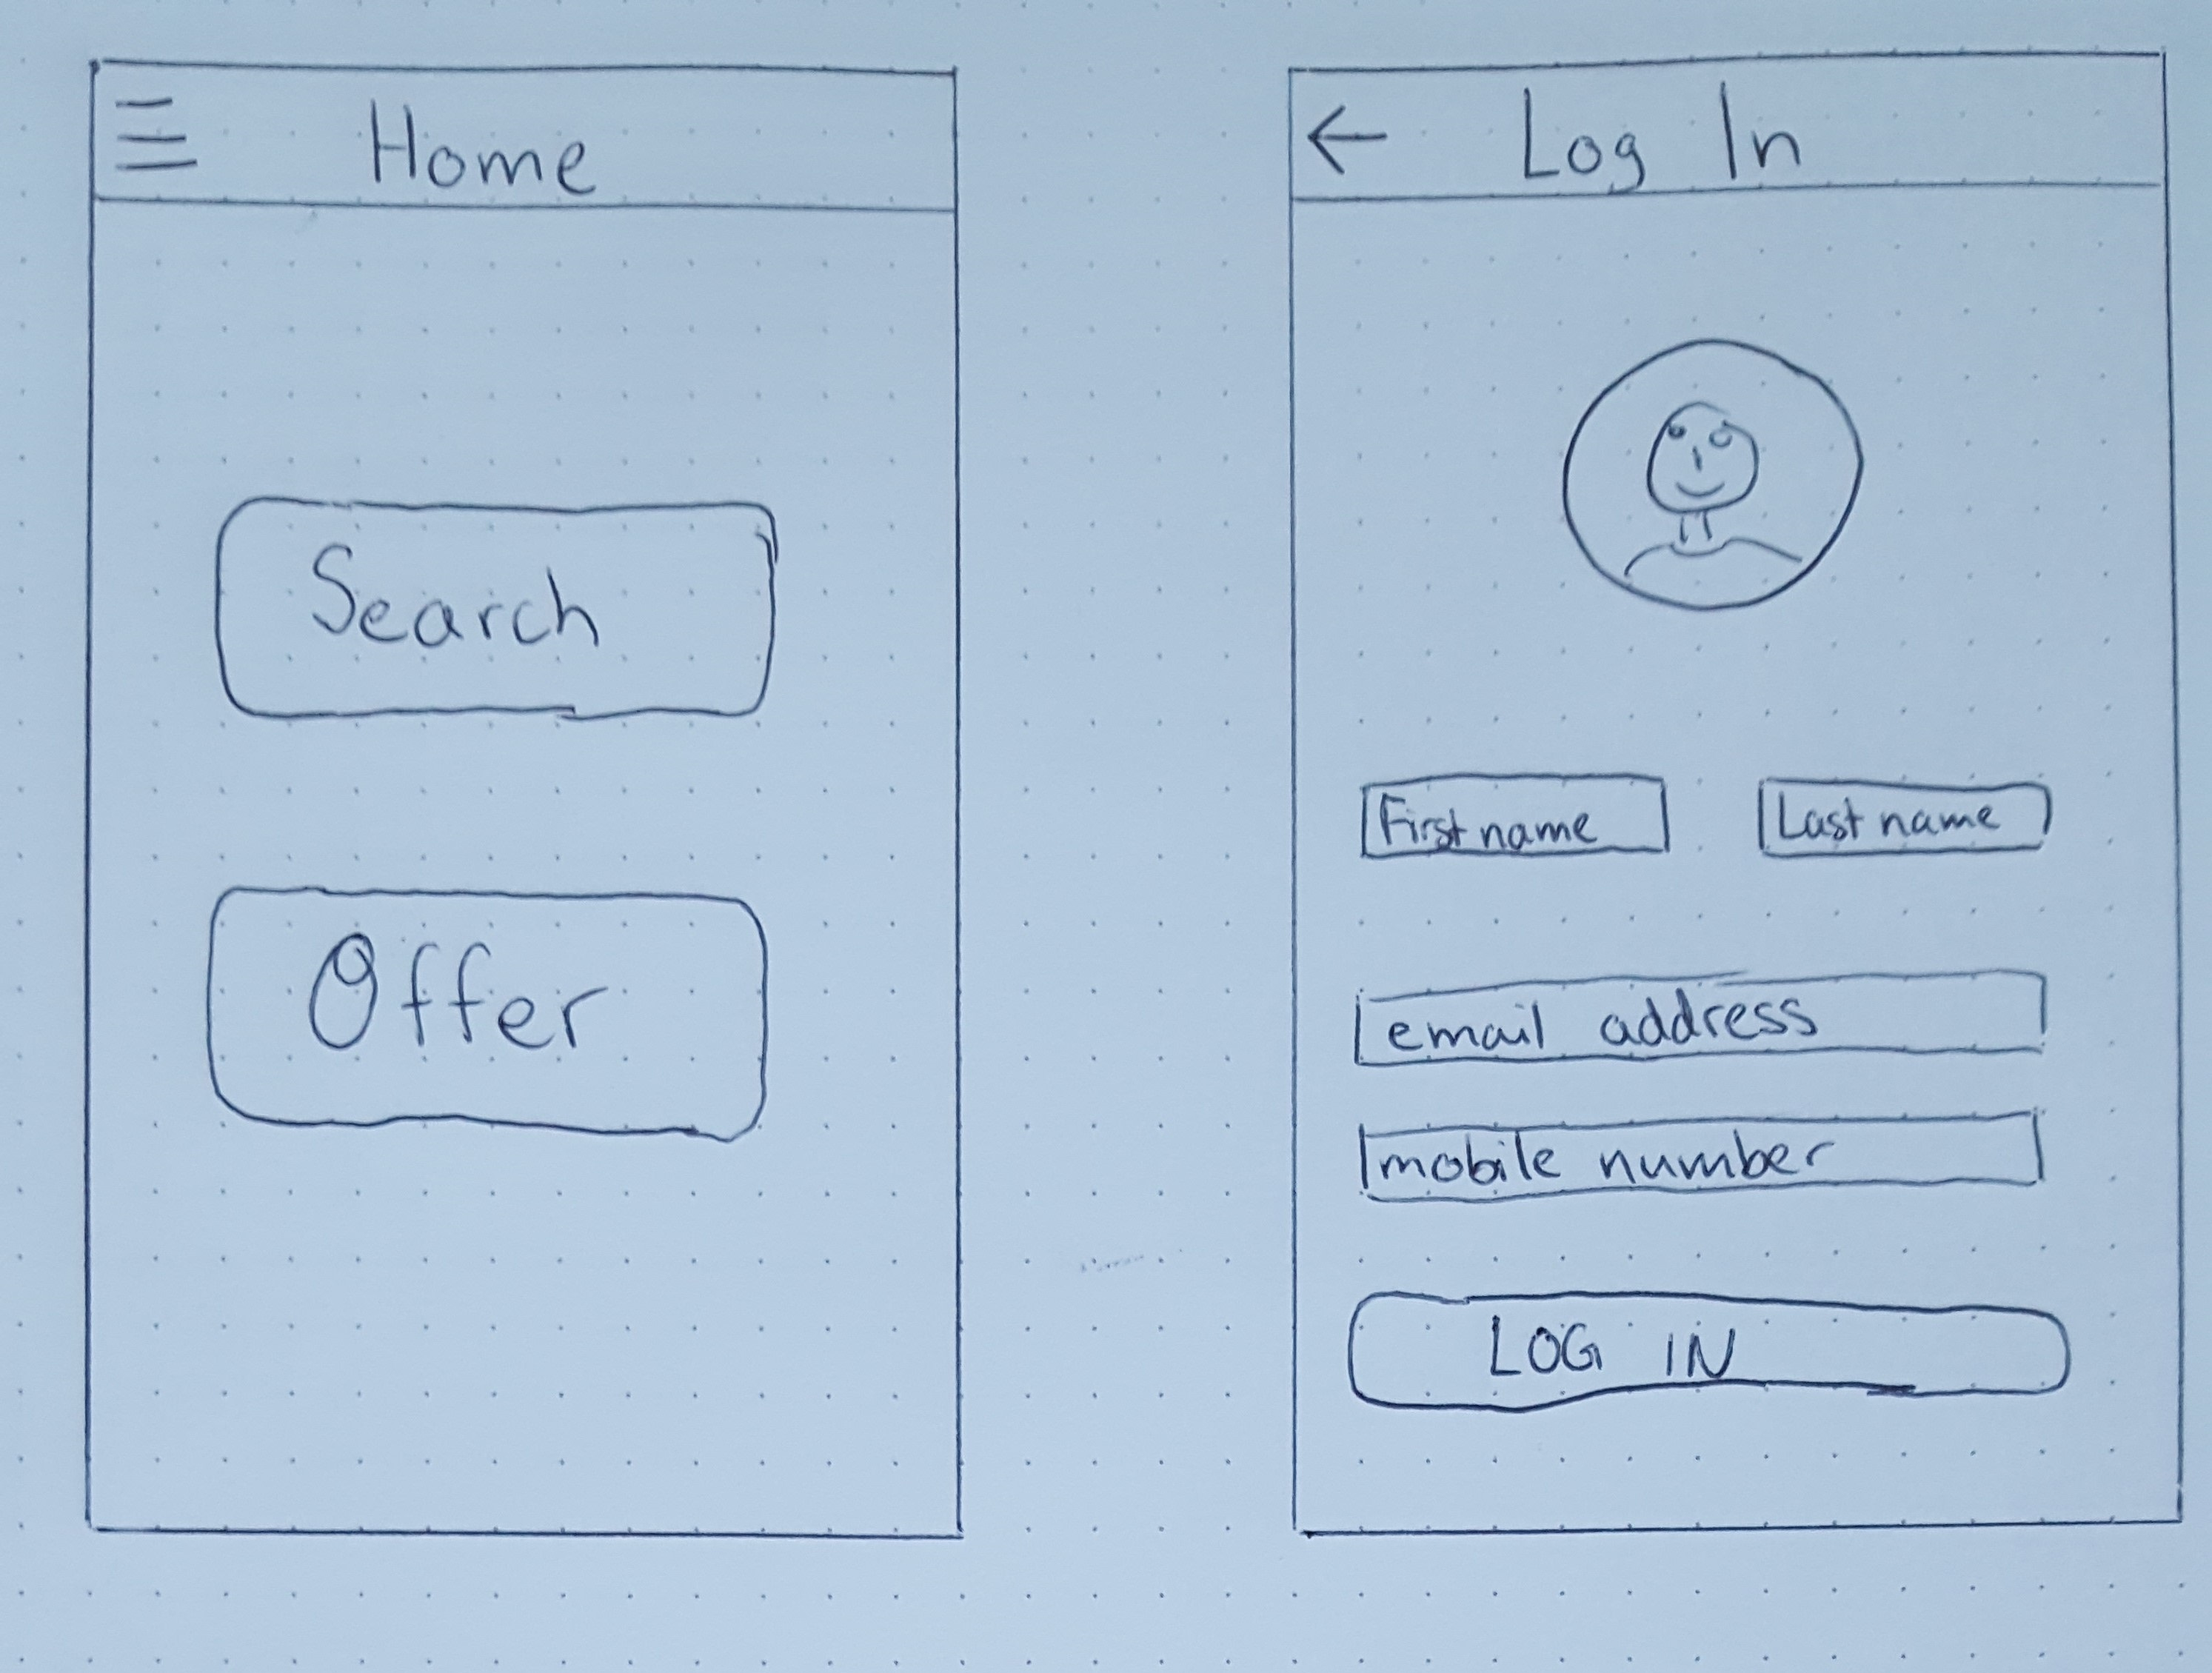
\includegraphics[width=0.8\linewidth]{jpg/paper-prototype-1-a}
\end{figure}
\end{frame}

%------------------------------------------------

\begin{frame}
\frametitle{Paper prototype}
\begin{figure}
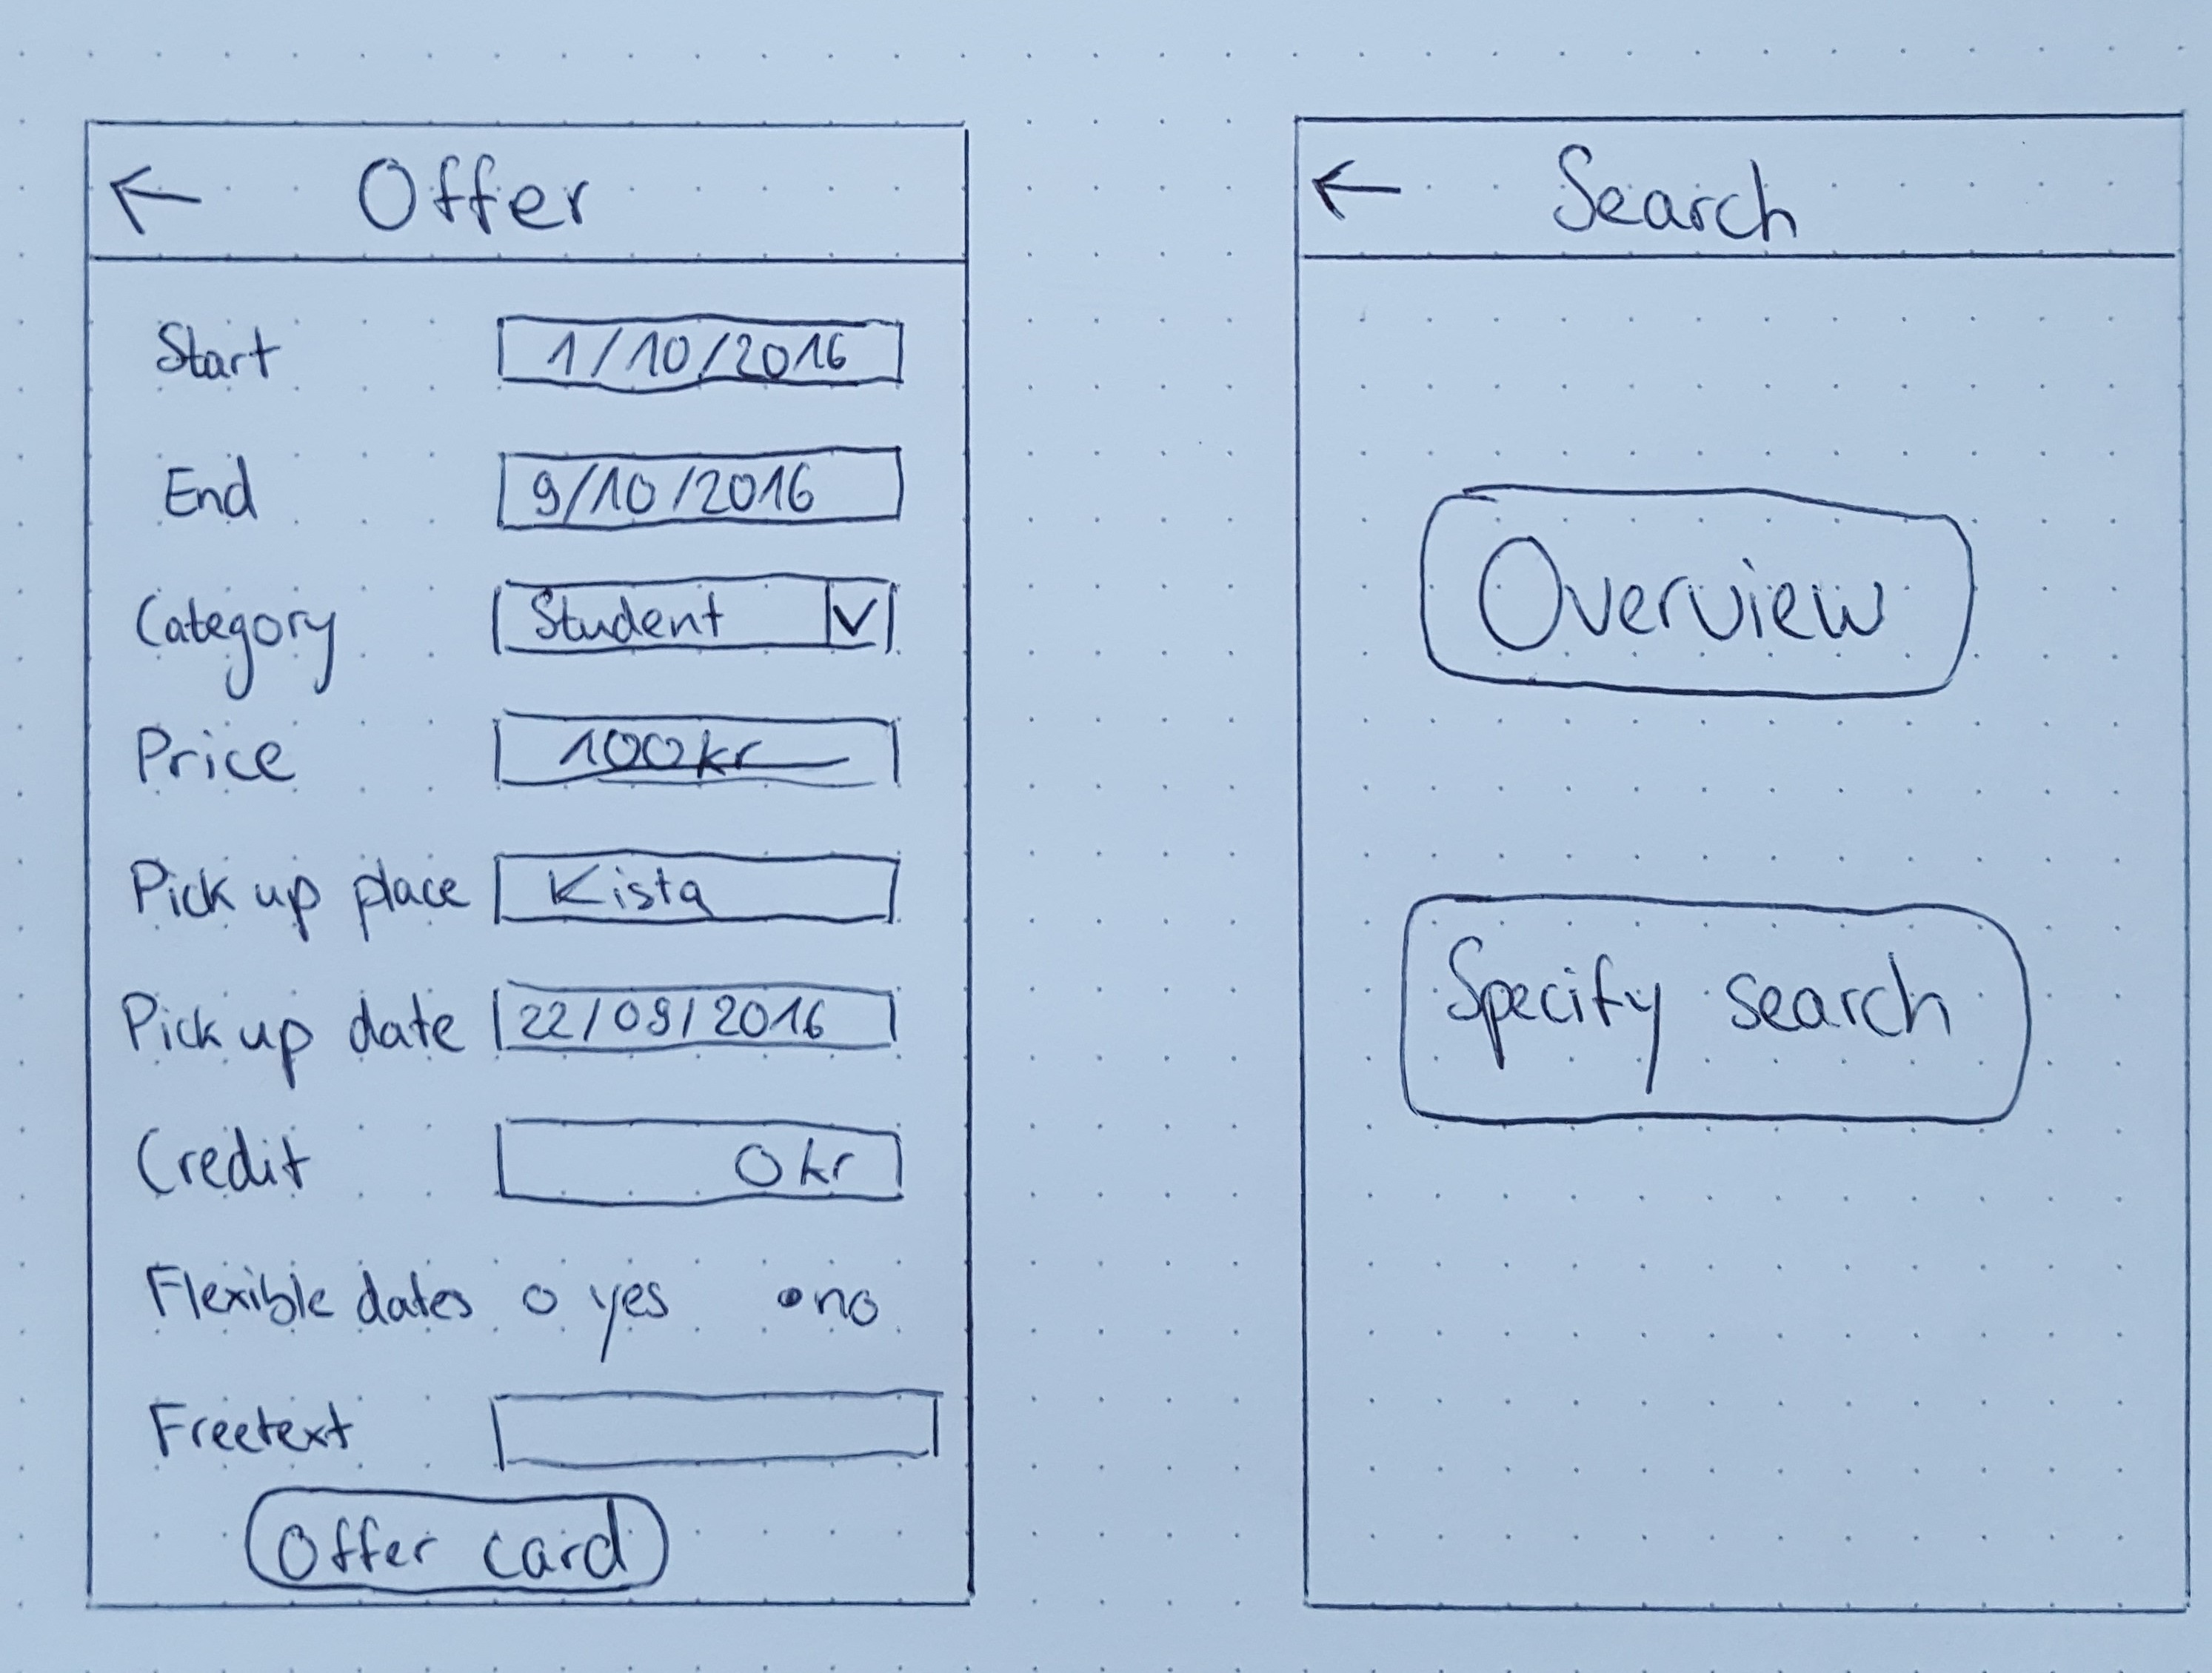
\includegraphics[width=0.8\linewidth]{jpg/paper-prototype-1-b}
\end{figure}
\end{frame}

%------------------------------------------------

\begin{frame}
\frametitle{Paper prototype}
\begin{figure}
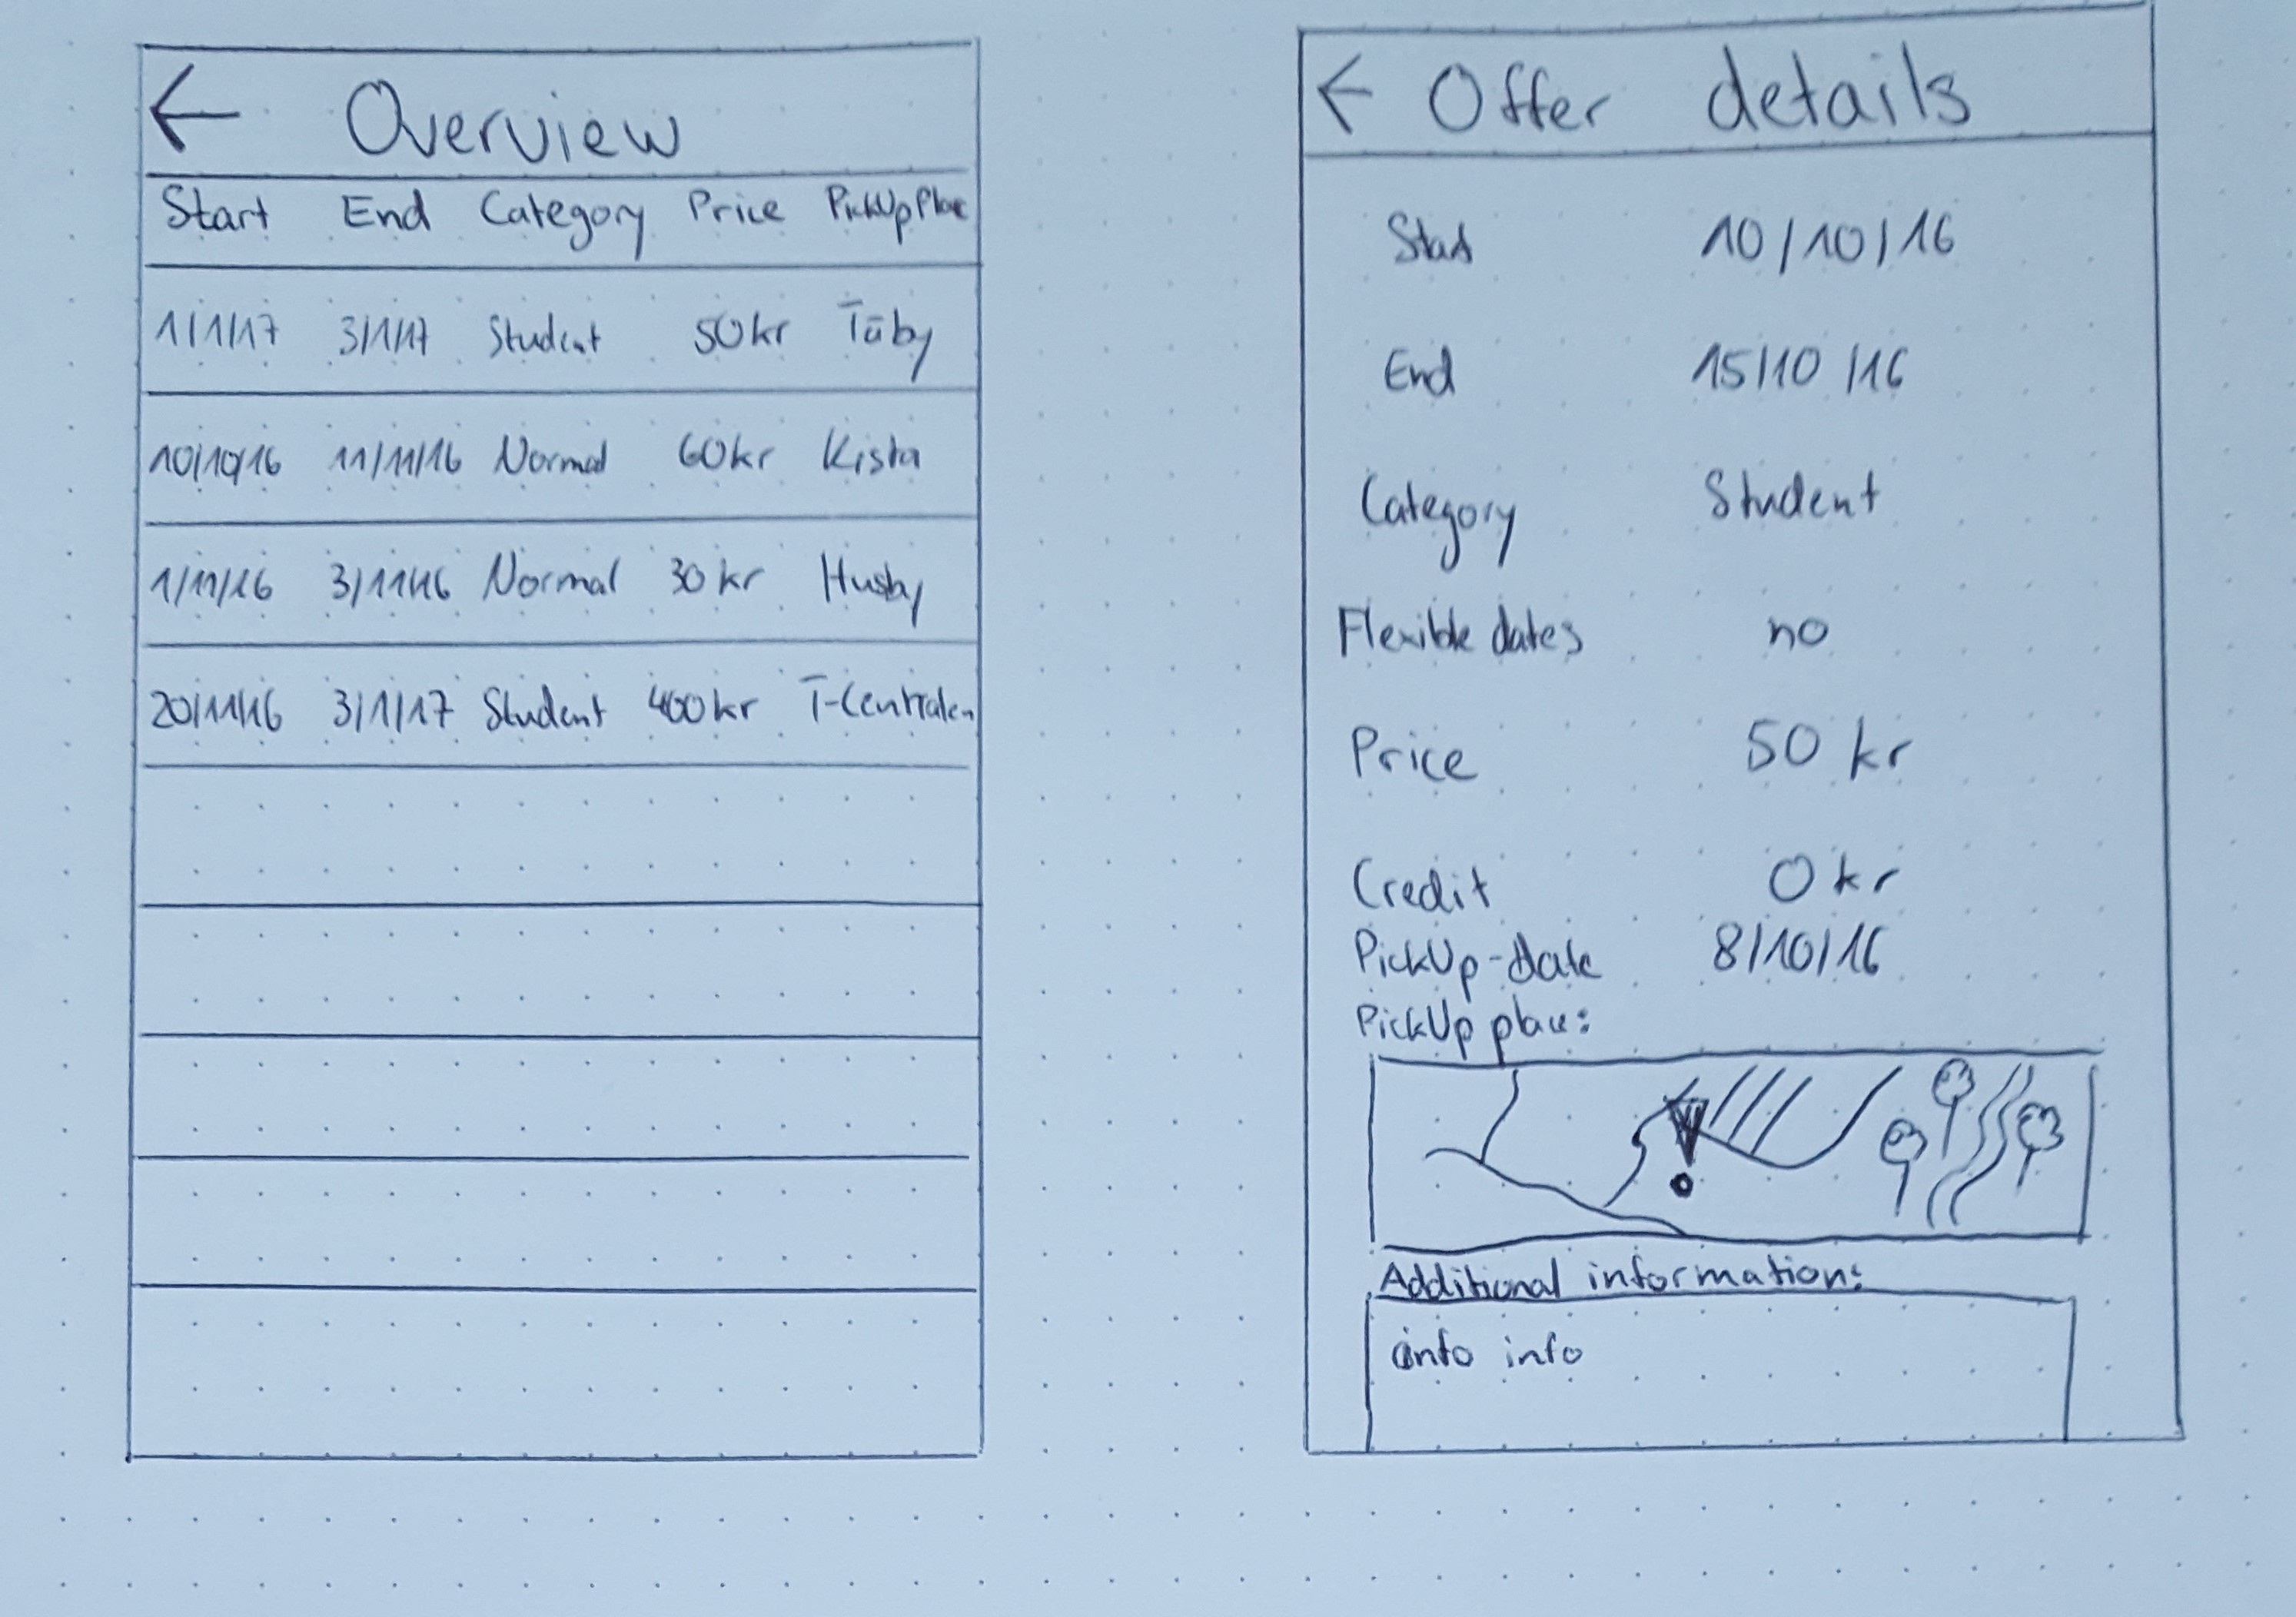
\includegraphics[width=0.8\linewidth]{jpg/paper-prototype-2-a}
\end{figure}
\end{frame}

%------------------------------------------------

\begin{frame}
\frametitle{Paper prototype}
\begin{figure}
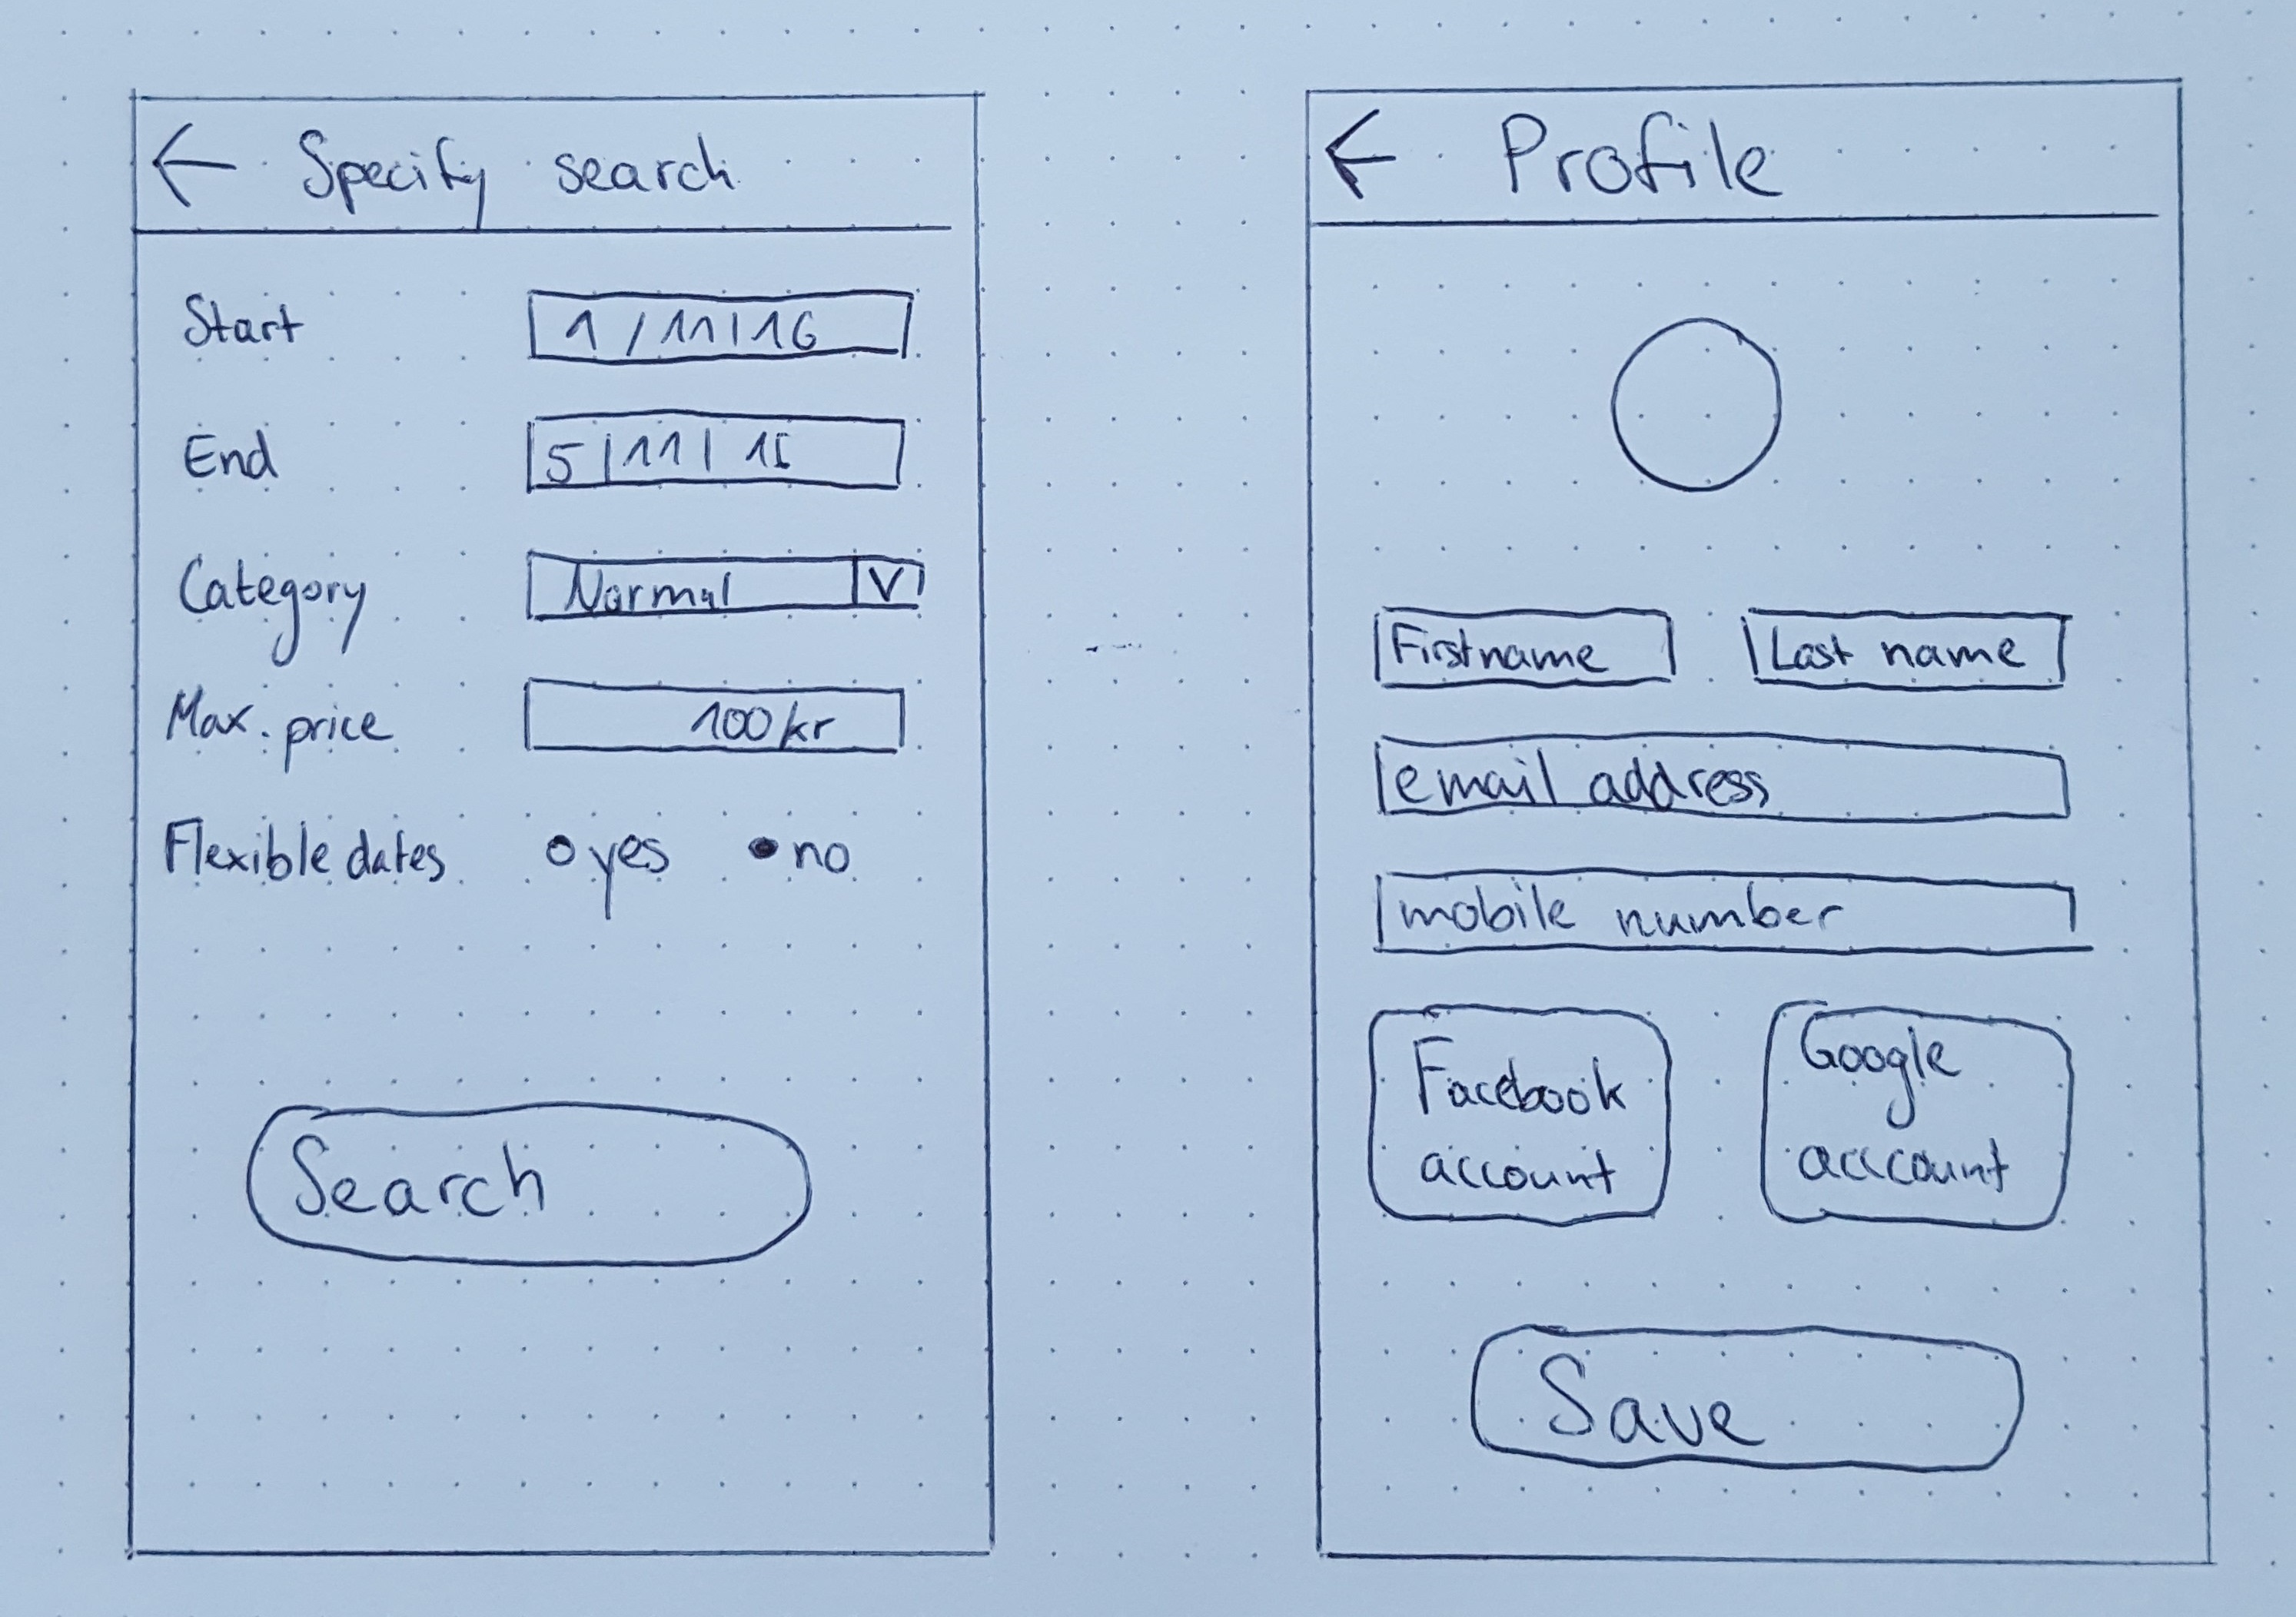
\includegraphics[width=0.8\linewidth]{jpg/paper-prototype-2-b}
\end{figure}
\end{frame}

%------------------------------------------------

\begin{frame}
\frametitle{Paper prototype feedback}
Name convention related:
\begin{itemize}
\item Change Free Text for Extra Information or Comment
\item Change Credit for Saldo
\item Change Pick Up Place for Pick Up Station
\end{itemize}
\end{frame}

%------------------------------------------------

\begin{frame}
\frametitle{Paper prototype feedback}
User interface related:
\begin{itemize}
\item Nice to have Start screen with the app logo
\item Nice to have an integrated chat system to contact the seller
\item Must have Log out button
\item Must have Support screen/tab for questions/feedback
\item Must have the insertion of the date with the popup calendar
\end{itemize}
\end{frame}

%------------------------------------------------

\begin{frame}
\frametitle{Paper prototype feedback}
Information related:
\begin{itemize}
\item Nice to have the suggested price for the given validity period
\item Must have Settings screen for date format and currency
\item Must have the user's contact information in Offer details 
\item Must have email address instead of phone number as user contact information

\end{itemize}
\end{frame}

%------------------------------------------------

\subsection{Site map} % A subsection can be created just before a set of slides with a common theme to further break down your presentation into chunks

%------------------------------------------------

\begin{frame}
\frametitle{Site map (using Balsamiq)}
\begin{figure}
\includegraphics[page=9,width=0.8\textwidth]{pdf/balsamiq}
\end{figure}
\end{frame}

%------------------------------------------------

\subsection{Click stream} % A subsection can be created just before a set of slides with a common theme to further break down your presentation into chunks

%------------------------------------------------

\begin{frame}
\frametitle{Click stream (using Balsamiq)}
\begin{figure}
\includegraphics[page=10,width=\textwidth]{pdf/balsamiq}
\end{figure}
\end{frame}

%------------------------------------------------

\subsection{WebApp prototype} % A subsection can be created just before a set of slides with a common theme to further break down your presentation into chunks

%------------------------------------------------

\begin{frame}
\frametitle{WebApp prototype (using Bootstrap)}
\begin{figure}
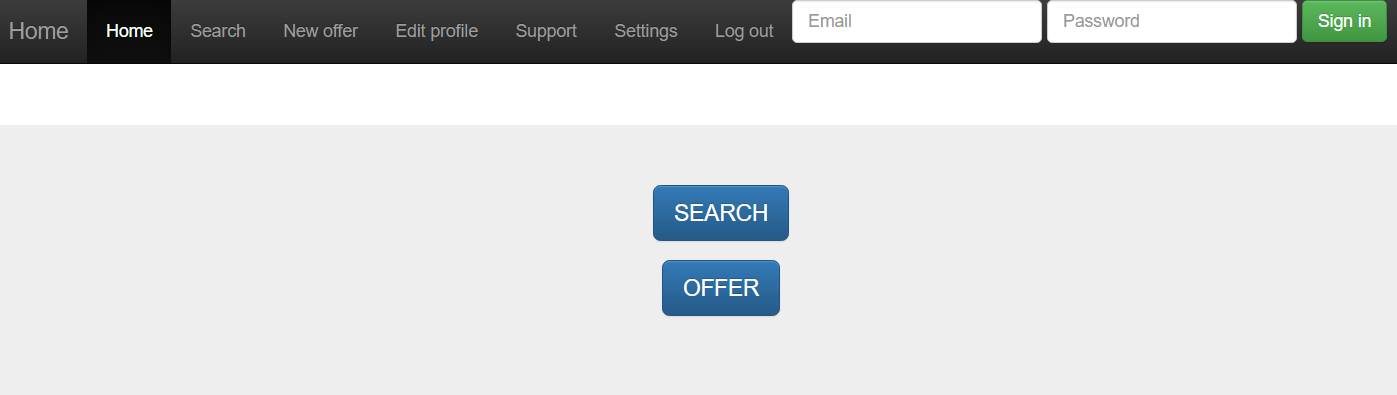
\includegraphics[width=\textwidth]{png/webapp-start.png}
\end{figure}
\end{frame}

%------------------------------------------------

\begin{frame}
\frametitle{WebApp prototype (using Bootstrap)}
\begin{figure}
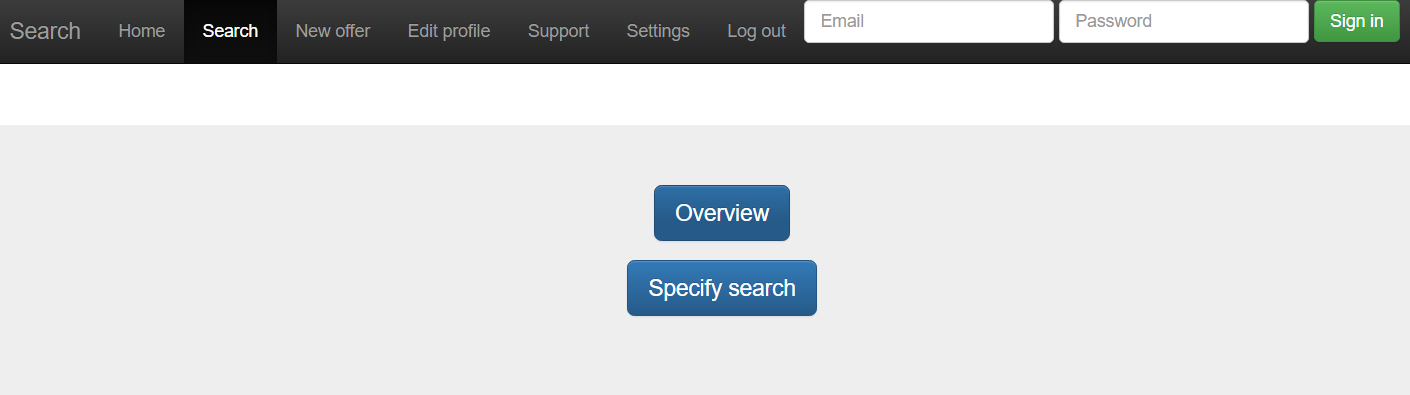
\includegraphics[width=\textwidth]{png/webapp-search.png}
\end{figure}
\end{frame}

%------------------------------------------------

\begin{frame}
\frametitle{WebApp prototype (using Bootstrap)}
\begin{figure}
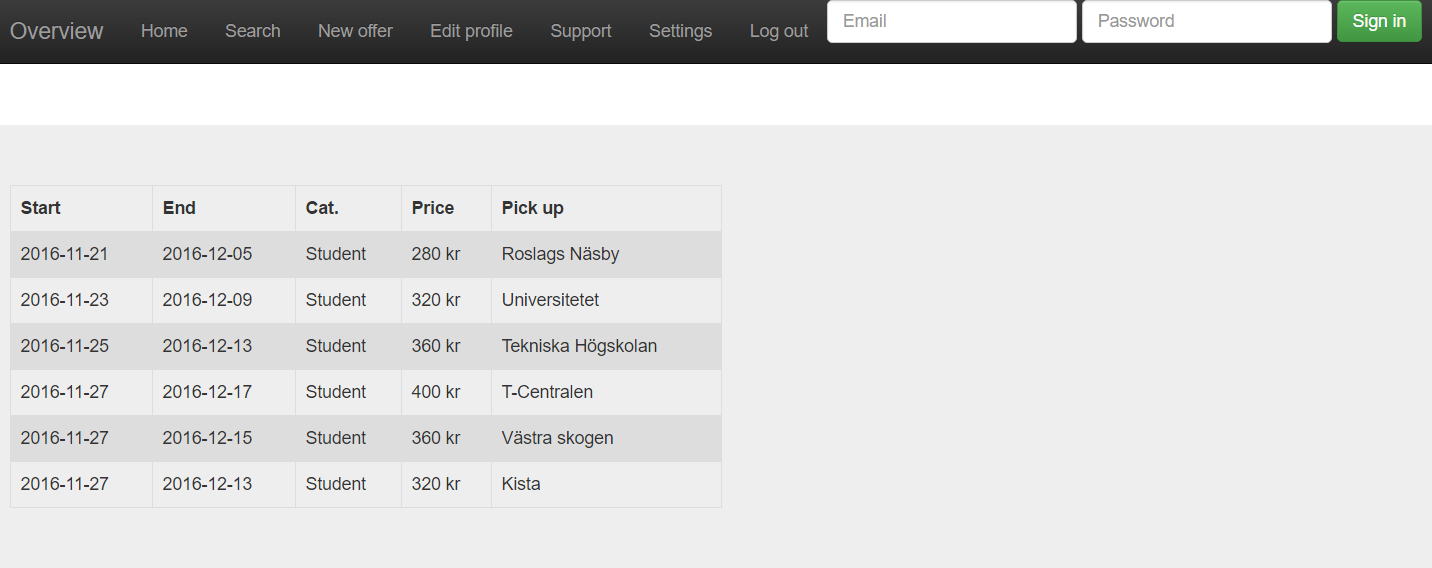
\includegraphics[width=\textwidth]{png/webapp-overview.png}
\end{figure}
\end{frame}

%------------------------------------------------

\begin{frame}
\frametitle{WebApp prototype (using Bootstrap)}
\begin{figure}
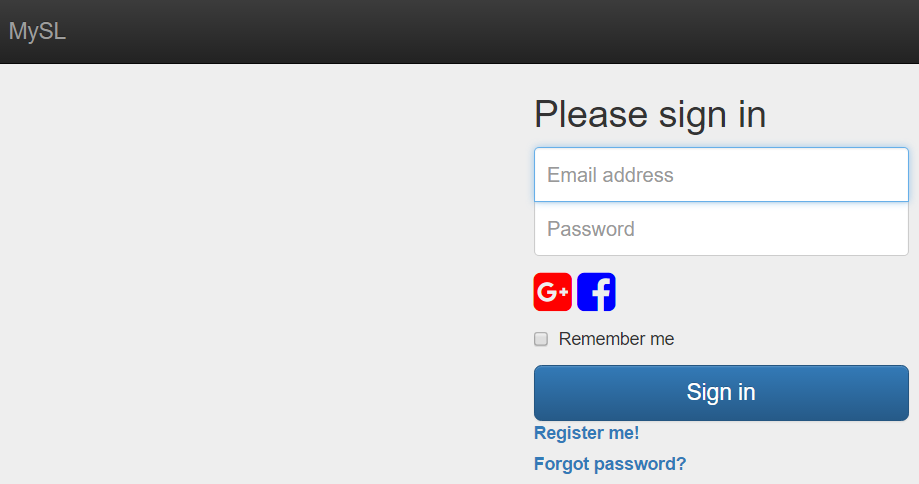
\includegraphics[width=\textwidth]{png/webapp-login.png}
\end{figure}
\end{frame}

%------------------------------------------------

\begin{frame}
\frametitle{WebApp prototype (using Bootstrap)}
\begin{figure}
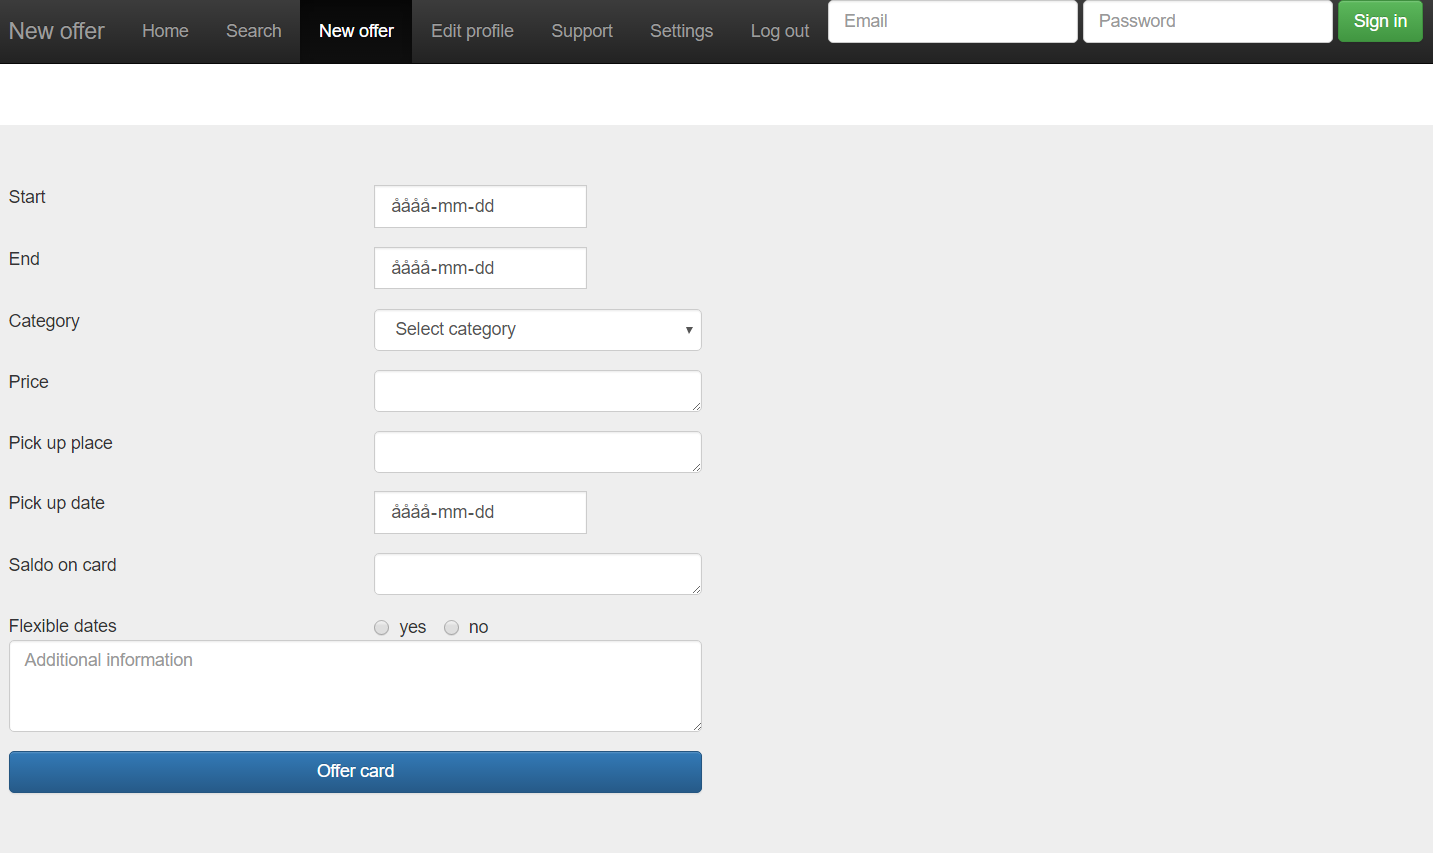
\includegraphics[width=\textwidth]{png/webapp-newoffer.png}
\end{figure}
\end{frame}

%------------------------------------------------

\begin{frame}
\frametitle{WebApp prototype (using Bootstrap)}
\begin{figure}
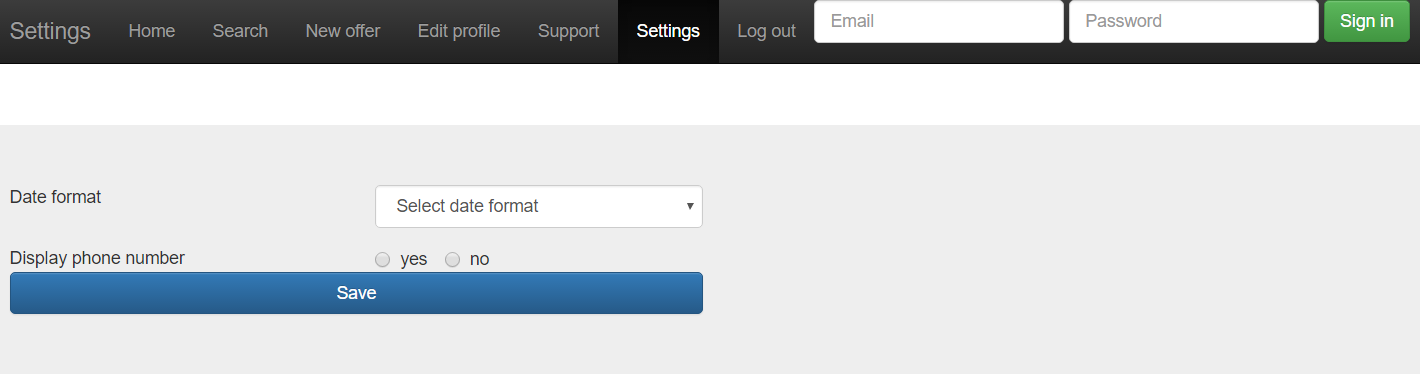
\includegraphics[width=\textwidth]{png/webapp-settings.png}
\end{figure}
\end{frame}

%------------------------------------------------

\subsection{Feedback} % A subsection can be created just before a set of slides with a common theme to further break down your presentation into chunks

%------------------------------------------------

\begin{frame}
\frametitle{WebApp prototype feedback}
\begin{itemize}
\item Offers should be clickable in search-overview menu
\item Put the calendar widget at the choice for the dates in Offer
\item Logging out should return to home
\item Offer in home and new offer in top menu: different outcomes
\end{itemize}
\end{frame}

%------------------------------------------------

\section{Android prototype}

%------------------------------------------------

\begin{frame}
\frametitle{Android prototype}
\begin{itemize}
\item Based on our WebApp prototype and its feedback
\item Developed using Android Studio
\item Used GitHub with Android integrated functionality ``VCS''
\item Used SourceTree as desktop client \& GUI for the repository
\item Each team member developed certain pages of the prototype
\item Implemented transition and connection between pages
\end{itemize}
\end{frame}

%------------------------------------------------

\subsection{Feedback} % A subsection can be created just before a set of slides with a common theme to further break down your presentation into chunks

%------------------------------------------------

\begin{frame}
\frametitle{Android prototype feedback}
\begin{itemize}
\item Buttons
\begin{itemize}
\item Text must be larger and/or in bold
\item Must be marked in a sharper color on bright light backgrounds
\item Search/offer look too similar to overview/specify search
\item Convenient to have a home button on all screens
\end{itemize}
\item Calendar
\begin{itemize}
\item Good to have the calendar so it is not necessary to type dates
\end{itemize}
\end{itemize}
\end{frame}

%------------------------------------------------

\subsection{Outlook} % A subsection can be created just before a set of slides with a common theme to further break down your presentation into chunks

%------------------------------------------------

\begin{frame}
\frametitle{Android prototype outlook}
\begin{itemize}
\item The map information shall be improved and implemented
\item The app logo should be seen on all screens
\item Home or back button on the top menu should be implemented
\end{itemize}
\end{frame}

%------------------------------------------------

\section{App web service}

%------------------------------------------------

\begin{frame}
\frametitle{App web service}
\begin{itemize}
\item Google Maps API
\begin{itemize}
\item Displays the location of the pick-up place
\end{itemize}
\item Facebook API
\begin{itemize}
\item Allows registration and login with Facebook
\item Enables integration and better customized service
\end{itemize}
\item SQLite API
\begin{itemize}
\item Relational database management system
\item Saves the data in a clear and managable manner
\end{itemize}
\end{itemize}
\end{frame}

%------------------------------------------------

\section{Demo}

%------------------------------------------------

\begin{frame}
\Huge{\centerline{Demo}}
\end{frame}

%----------------------------------------------------------------------------------------

\end{document} 